%++++++++++++++++++++++++++++++++++++++++
% Don't modify this section unless you know what you're doing!
\documentclass[letterpaper,12pt]{article}
\usepackage{tabularx} % extra features for tabular environment
\usepackage{amsmath}  % improve math presentation
\usepackage{graphicx} % takes care of graphic including machinery
\usepackage[margin=1in,letterpaper]{geometry} % decreases margins
\usepackage{cite} % takes care of citations
\usepackage[latin9]{inputenc}
\usepackage{lmodern} % for writing code
\usepackage{tikz}
\usetikzlibrary{positioning,shapes.geometric}
\usepackage{minted}
\usepackage{amsfonts}



\usepackage[final]{hyperref} % adds hyper links inside the generated pdf file
\hypersetup{
	colorlinks=true,       % false: boxed links; true: colored links
	linkcolor=blue,        % color of internal links
	citecolor=blue,        % color of links to bibliography
	filecolor=magenta,     % color of file links
	urlcolor=blue         
}
\definecolor{ao(english)}{rgb}{0.0, 0.5, 0.0}
\usepackage{xcolor}
\renewcommand{\labelitemi}{$\bullet$}
\renewcommand{\labelitemii}{$\cdot$}
\renewcommand{\labelitemiii}{$\diamond$}
\renewcommand{\labelitemiv}{$\ast$}
%\usepackage[usenames,dvipsnames,svgnames,table]{xcolor}
%\let\oldtriangleleft\triangleleft
%\DeclareRobustCommand\bowtie{\mathrel\triangleright\joinrel\mathrel\oldtriangleleft}


%++++++++++++++++++++++++++++++++++++++++


\begin{document}

\title{Software Verification\\
Implementing a bounded model-checker}
\author{Ida Tucker}
\date{\today}
\maketitle

\begin{abstract}
The goal of this homework is to implement a bounded model-checker based on a depth-first-search exploration of all the feasible paths
of the input program. The SMT-solver Z3 is used as an
execution engine to compute all the successive states along the exploration. In this report is first described how operators of the program are translated into Z3 propositional formulas via the module \texttt{Semantics.ml}. Then the logic behind the implementation of the bounded model checker is laid out and finally a series of additional test cases are explained, with actual and expected results.
\end{abstract}


\section{Implementation of Semantics.ml}
\paragraph{}
The \texttt{Semantics.ml} module translates the operators of the program into Z3 expressions in the integer theory module.
\subsection{Keeping track of formulas added to the Z3 expression}
\paragraph{}
In order to keep track of the formulas associated to each variable, a hashtable, global to the module, which is reset for every new transition, is used. This hashtable \texttt{\textcolor{blue}{ht}} binds the indexed program variables to the appropriate formula.
Separate keys are added if the formula is asserting that a variable is non zero. These keys are of the form \textcolor{purple}{\texttt{x\$i-non-zero}}.
If the program operation is a guard, the hashtable has one additional key \textcolor{purple}{\texttt{guard}} since the formula for the guard exists alongside formulas added for each variable. Moreover we will only have one guard formula per operation.
\paragraph{}
Using a hashtable enables us to avoid the duplication of formulas associated to a given variable and to easily update them without having to check their existence. 
\paragraph{}
Thus the keys in the hashtable are:
\begin{itemize}
\item $\forall x \in X$,  \textcolor{purple}{x\$i}
\item $\forall x \in X$ such that we require $x \neq 0$, \textcolor{purple}{x\$i-non-zero}
\item if \textit{op} is a guard, \textcolor{purple}{guard}
\end{itemize}

\subsection{Defining propositional formulas}
\paragraph{}
Now we have established how to keep track of the added formulas, let us see how they are built.

The commands are our program operations. In order to transform the program operation into a list of formulas we first need to determine what command is being applied.
Therefore, the \texttt{formula} method pattern matches the input command \texttt{\textcolor{olive}{cmd}} with the appropriate sort. According to the the matched sort, the appropriate function \texttt{apply\_skip}, \texttt{apply\_guard} or \texttt{apply\_assign} is called. 


\begin{minted}{ocaml}
  match cmd with
  | Command.Skip ->
     List.iter (apply_skip ctx  i) vars;
     Hashtbl.fold (fun _ v acc -> v :: acc) ht []
  | Command.Guard p ->
     apply_guard ctx p i vars;
     Hashtbl.fold (fun _ v acc -> v :: acc) ht []
  | Command.Assign (v, e) ->
     apply_assign ctx (v,e) i vars;
     Hashtbl.fold (fun _ v acc -> v :: acc) ht []
\end{minted}

If the program operation is a \textit{skip}, since the same formula will be applied to each variable we simply iterate through each variable in \texttt{\textcolor{olive}{vars}} and apply skip. The \texttt{apply\_skip} method is called on a single variable, it ensures that the variable remains unchanged from index $i$ to index $i+1$ by adding a new formula to \texttt{\textcolor{blue}{ht}} associated to $x^{(i)}$:
$$ x^{(i)} == x^{(i+1)} $$

The addition of the formula to \texttt{\textcolor{blue}{ht}} is done in the method \texttt{add\_unchanged}.
\paragraph{}
The \texttt{apply\_guard} and \texttt{apply\_assign} methods, which are applied if the program operation is a \textit{guard} or an \textit{assignment} are detailed below in \ref{guard} and \ref{assign}.
They both also update the hashtable and return the sort \texttt{unit}.
\paragraph{}
Whatever the program operation, after the appropriate function has been called, we iterate through the hashtable to build the returned list of formulas.

\subsection{Program operation is a guard}\label{guard}
If the command is a guard it is defined as follows:
\begin{align*}
op^{(i)} = g^{(i)} \wedge \bigwedge_{y \in X}(y^{(i+1)} = y^{(i)})
\end{align*}
And $ g^{(i)} = e_1^{(i)} \sim e_2^{(i)}$ where  $\sim$ is an operator in $ \{ = ,\leq, < , >, \geq \}$  

\paragraph{}
To satisfy this definition, a formula is added to the hashtable \texttt{\textcolor{blue}{ht}} for the guard $g$, and for each variable we ensure that the variable remains unchanged from index $i$ to index $i+1$. 
Ensuring variables remain unchanged is equivalent to calling \texttt{apply\_skip} on all variables.
Thus the \texttt{apply\_guard} function first adds a formula for the guard, before iterating through each variable in \texttt{\textcolor{olive}{vars}}  and applying \texttt{apply\_skip}.

In order to build the guard formula, the \texttt{eval} function evaluates expressions $e_1^{(i)}$ and $e_2^{(i)}$ recursively, in order to build formulas in the Z3 context for the expressions. The \texttt{eval} function takes care of adding a \texttt{\textcolor{purple}{non-zero}} key to \texttt{\textcolor{blue}{ht}} if the expression includes a division by a constant, a program variable, or an expression including program variables.

\subsection{Program operation is an assignment}\label{assign}

If the command is an assignment we have:
\begin{align*}
op^{(i)} = (x^{(i+1)} = e^{(i)}) \wedge \bigwedge_{y \in X\backslash \{x\} }(y^{(i+1)} = y^{(i)})
\end{align*}

All variables should remain unchanged from index $i$ to index $i+1$ \textit{except} the variable that is being assigned to. Thus \texttt{apply\_assign} iterates through each variable in \texttt{\textcolor{olive}{vars}} and applies \texttt{apply\_skip} before adding a formula for the assignment associated with $x^{(i)}$, which will replace the previous binding of $x^{(i)}$ in \texttt{\textcolor{blue}{ht}}.
i.e. the binding \{\texttt{\textcolor{purple}{x\$i}}, $x^{(i)}$ = $x^{(i+1)}$\} becomes \{\texttt{\textcolor{purple}{x\$i}}, $x^{(i+1)} = e^{(i)}$\}.

In order to build the assignment formula the expression assigned to $x^{(i)}$ is matched with either a constant, another variable or an expression. Again if $e^{(i)}$ is an expression we use the \texttt{eval} function to evaluate the expression.

\subsection{Testing division by zero} 
Tests have been added to \texttt{Test\_Semantics.ml} for the division by zero.

\paragraph{Test 1:}division of an expression by a constant
\paragraph{Expected result:}a formula should be added asserting the integer constant is non zero.
\paragraph{Obtained result:}
\begin{minted}{ocaml}
[z := (x / 2)]^1: expects `{(= z$2 (div x$1 2)), (= x$1 x$2),
				(= y$1 y$2), (not (= 2 0))}'
\end{minted}
\textcolor{teal}{PASS}

\paragraph{Test 2:}division of an expression by an expression that is neither a constant nor a variable.
\paragraph{Expected result:}a formula should be added asserting the expression is non zero.
\paragraph{Obtained result:}
\begin{minted}{ocaml}
[z := (x / (y + 3))]^1: expects `{(= z$2 (div x$1 (+ y$1 3))), (= x$1 x$2),
				(= y$1 y$2), (not (= (+ y$1 3) 0))}'
\end{minted}
\textcolor{teal}{PASS}

\paragraph{Test 3:}division of an expression by a more complex expression.
\begin{minted}{ocaml}
z := x / ((y * cst 2) + (y / (x + y))) 
\end{minted}
\paragraph{Expected result:}formulas should be added asserting the relevant expressions are non zero.
\paragraph{Obtained result:}an unexpected variable \texttt{a!1} is introduced, but presumably this is the way the Z3 solver deals with such expressions. Nevertheless the obtained result is correct.
\begin{minted}{ocaml}
[z := (x / ((y * 2) + (y / (x + y))))]^1: expects `{(let ((a!1 (div x$1 
	(+ ( * y$1 2) (div y$1 (+ x$1 y$1)))))) (= z$2 a!1)),
    (let ((a!1 (= (+ ( * y$1 2) (div y$1 (+ x$1 y$1))) 0))) (not a!1)),
    (= x$1 x$2), (= y$1 y$2), (not (= (+ x$1 y$1) 0))}'
\end{minted}

\textcolor{teal}{PASS}


\section{Implementation of BoundedModelChecking.ml}
\subsection{Marking locations as visited}
Since the constraints associated to a location evolve as we propagate the search, this implementation of a depth first search does not mark the nodes as visited. If we were to mark them as visited we would need to ensure we have encountered a fixed point.


\subsection{Keeping track of path and depth of search}

\begin{itemize}
\item The global variable \texttt{depth} is incremented every time we apply \texttt{depth\_first\_search} to a child node.
\item The global variable \texttt{path} is a list of pairs \texttt{(command, location)} that keeps track of the edges of the CFA taken to get to the current location.
\item The global variable \texttt{bad\_path} is a list of pairs \texttt{(command, location)} that lead to the final location, if such a path of depth lower than \texttt{bound} exists. If no such path exists (or has been discovered yet) \texttt{bad\_path} is the empty list.
\item \texttt{bound\_reached} is a Boolean, initially set to \texttt{false}, to which we assign the value \texttt{true} if there exists a path along which the bound is reached before encountering the final location or an unreachable location.
\end{itemize}


\subsection{Building the path and the path formula}
\paragraph{}
Every time a new branch of the CFA is explored, the \texttt{depth\_first\_search} function checks if \texttt{bad\_path} is empty, if not it returns. 

If \texttt{bad\_path} is empty, it checks if the \texttt{bound} has been reached, if so it returns.

Otherwise we are in the valid situation where the program should continue the depth first search. In this situation the following logic is applied:

\begin{itemize}
\item Increase depth by one.
\item Create a new scope for the solver by saving the current stack size: pushing the solver will enable us to backtrack later on if we reach the \texttt{bound} or an unfeasible path.
\item Call \texttt{\textcolor{blue}{Semantics.}formula} on the program operation for the current depth in order to convert the command into a propositional logic formula.
\item Add the formula to the solver.
\item Add the pair \texttt{(command, location)} to the \texttt{path} list.
\item Check the satisfiability of the solver. At this point, three situations may arise:
\begin{enumerate}
\item{The solver is not satisfiable, in which case we backtrack:
\begin{itemize}
\item restore the previous context by popping the solver
\item decrease the depth by one
\item remove the pair \texttt{(command, location)} last added to \texttt{path}
\item return \texttt{unit}.
\end{itemize}
}
\item The solver is satisfiable and we have reached the final location. In this case we assign \texttt{path} to \texttt{bad\_path} and return \texttt{unit}.
\item The solver is satisfiable, thus the location is reachable, and the location is not the final location. In this situation we iterate through all locations accessible from the current location and apply \texttt{\textcolor{blue}{depth\_first\_search}}.
\end{enumerate}
\end{itemize}

\subsection{Searching for a path to the final state}
\paragraph{}
The \texttt{\textcolor{blue}{search}} function brings all the above functionality together.
It first initialises the global variables before calling \texttt{\textcolor{blue}{depth\_first\_search}} on the initial location with the command skip.

If after calling \texttt{\textcolor{blue}{depth\_first\_search}} the \texttt{bad\_path} list is not empty, then the depth first search found a feasible path to the final location and the \texttt{Path bad\_path} is returned.

If no path to the final state is found, but the bound has been reached, the program may not be safe, we only know that there is no path to the final state in less than \texttt{bound} steps. In this case the \texttt{bound\_reached} variable is true, and \texttt{Empty \textcolor{teal}{false}} is returned.

Otherwise, all feasible paths of have been explored and none lead to the final state. The program is safe and \texttt{Empty \textcolor{teal}{true}} is returned.


\section{Tests}
The test cases described bellow all take as input an automaton (from the \texttt{examples} directory), and expect an output of type \texttt{result}:
\begin{itemize}
\item a \texttt{Path} p where p is a feasible path of the automaton leading to the final state of length at most \texttt{bound}
\item no feasible path
\item no feasible path of length at most \texttt{bound}
\end{itemize}

\subsection{New Automatons}
The additional automatons created in the \texttt{examples} folder test edge cases, the case where no feasible path is found in less than 10 iterations, unsafe programs, potential infinite loops etc.

\subsubsection{Initial state is bad state}
\paragraph{Test File:} \texttt{init\_is\_final.aut}
\paragraph{Test}
Edge case where the initial and final location are the same node.
\paragraph{Expected result}
A feasible path that is simply the initial location (no commands).
\paragraph{Obtained result}
\textbf{\textcolor{teal}{PASS}}


\subsubsection{Initial state skips to bad state}
\paragraph{Test File:} \texttt{init\_skip\_final.aut }
\paragraph{Test}
Edge case where the initial location skips to the final location.
\paragraph{Expected result}
A feasible path that is simply a skip from the initial location to the final location.
\paragraph{Obtained result}
\textbf{\textcolor{teal}{PASS}}

\subsubsection{\texttt{bound} is 0}

\paragraph{Test}
Test the edge case where the bound is zero and the final location is not the initial location.
\begin{minted}{ocaml}
./bmc.d.byte -bound 0 examples/init_skip_final.aut 
\end{minted}
\paragraph{Expected result}
No feasible path of length $\leq 0$.
\paragraph{Obtained result}
\begin{minted}{vctreestatus}
No feasible path of length <= 0
\end{minted}
\textbf{\textcolor{teal}{PASS}}


\paragraph{Test}
Test the edge case where the bound is zero and the final location is the initial location.
\begin{minted}{ocaml}
./bmc.d.byte -bound 0 examples/init_is_final.aut 
\end{minted}
\paragraph{Expected result}
A feasible path that is simply the initial location (no commands).
\paragraph{Obtained result}
\begin{minted}{vctreestatus}
Feasible path:   q_0
\end{minted}
\textbf{\textcolor{teal}{PASS}}




\subsubsection{Looping until reaching the final location}\label{loop-to-final}

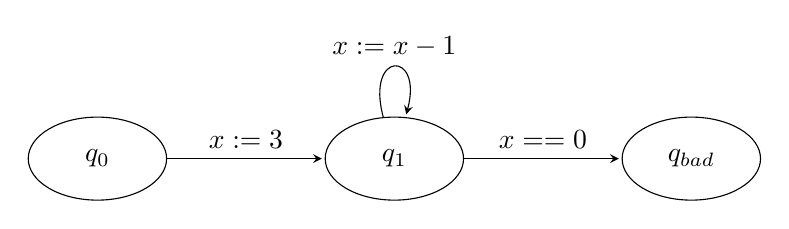
\begin{tikzpicture}[%
    ->,shorten >=1pt,>=stealth,node distance=7cm,noname/.style={%
      ellipse,minimum width=5em, minimum height=3em,draw}
  ]
    \node[noname] (ini)                                                {$q_{0}$};
    \node[noname] (1) [node distance=2cm, right=of ini]    {$q_{1}$};
    \node[noname] (bad) [node distance=2cm, right=of 1]   {$q_{bad}$};
    \path (ini) edge [above]                  node {$x:=3$} (1)
    	  (1)   edge [loop above]             node {$x:=x-1$} (1)
          (1)   edge [above]                  node {$x==0$} (bad)
          ;
\end{tikzpicture}
  
\paragraph{Test File:} \texttt{loop\_location\_bad.aut}
\paragraph{Test:}
Ensure the program will loop on a single state in order to reach the final node.
\paragraph{Expected result:}
A path to the final state.
\paragraph{Obtained result:}
\begin{minted}{ocaml}
Feasible path:
   q_0
      >> x := 5 >>
   q_1
      >> x := (x - 1) >>
   q_1
      >> x := (x - 1) >>
   q_1
      >> x := (x - 1) >>
   q_1
      >> x == 0 >>
   q_2

\end{minted}
\textbf{\textcolor{teal}{PASS}}


\subsubsection{Limit under and limit over \texttt{bound}}
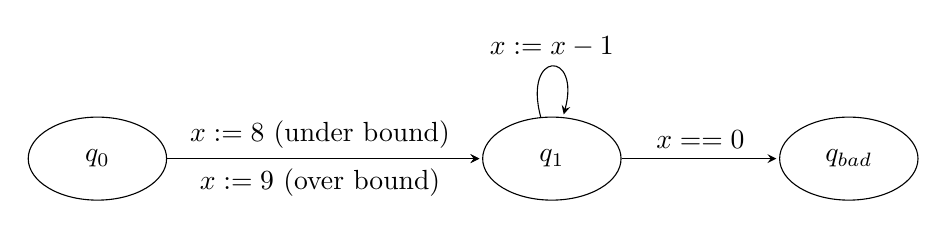
\begin{tikzpicture}[%
    ->,shorten >=1pt,>=stealth,node distance=7cm,noname/.style={%
      ellipse,minimum width=5em, minimum height=3em,draw}
  ]
    \node[noname] (ini)                                                {$q_{0}$};
    \node[noname] (1) [node distance=4cm, right=of ini]    {$q_{1}$};
    \node[noname] (bad) [node distance=2cm, right=of 1]   {$q_{bad}$};
    \path (ini) edge [above]                  node {$x:=8 \mbox{ (under bound) }$} (1)
    	  (ini) edge [below]                  node {$x:=9 \mbox{ (over bound) }$} (1)
    	  (1)   edge [loop above]             node {$x:=x-1$} (1)
          (1)   edge [above]                  node {$x==0$} (bad)
          ;
  \end{tikzpicture}
  
\paragraph{Test Files:} \texttt{limit\_under\_bound.aut}, \texttt{limit\_over\_bound.aut}
 
\paragraph{Test:}
\texttt{bound} is 10 and:
\begin{enumerate}
\item the CFA requires exactly 10 steps to the bad state.
\item the CFA requires exactly 11 steps to the bad state
\end{enumerate}
\paragraph{Expected result:}
\begin{enumerate}
\item A path to the final state.
\item No feasible path of length $\leq 10$.
\end{enumerate}
\paragraph{Obtained result:}
\textbf{\textcolor{teal}{PASS}}

  
  
  
  
\subsubsection{Always negative}
\paragraph{Test File:} \texttt{always\_negative.aut}
\paragraph{Test} The following CFA

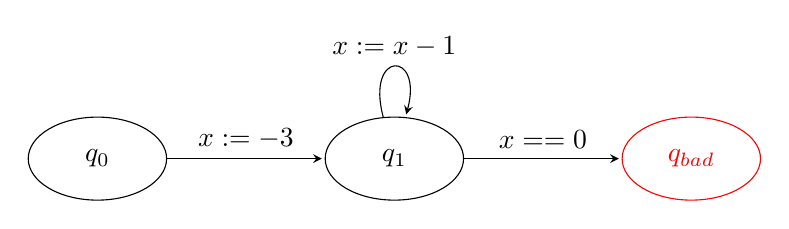
\begin{tikzpicture}[%
    ->,shorten >=1pt,>=stealth,node distance=7cm,noname/.style={%
      ellipse,minimum width=5em, minimum height=3em,draw}
  ]
    \node[noname] (ini)                                        {$q_{0}$};
    \node[noname] (1) [node distance=2cm, right=of ini]        {$q_{1}$};
    \node[noname, red] (bad) [node distance=2cm, right=of 1]   {$q_{bad}$};
    \path (ini) edge [above]                  node {$x:=-3$}  (1)
    	  (1)   edge [loop above]             node {$x:=x-1$} (1)
          (1)   edge [above]                  node {$x==0$}   (bad)
          ;
  \end{tikzpicture}

\paragraph{Expected result:}
No path to the final state should be found, since we have a safe inductive invariant:
\begin{itemize}
\item $\varphi _{q_0}$ = true
\item $\varphi _{q_1}$ = $ x < 0$
\item $\varphi _{q_{bad}}$ = false
\end{itemize}
\paragraph{Obtained result:}
The bounded model checker does not guarantee the safety of the the program but whatever the \texttt{bound} set, it finds no feasible path of length $\leq$ \texttt{bound}.\\
\textbf{\textcolor{teal}{PASS}}

\subsubsection{Unsafe program}
\paragraph{Test File:} \texttt{unsafe\_program.aut}
\paragraph{Test}
Slightly more complex unsafe program:\\
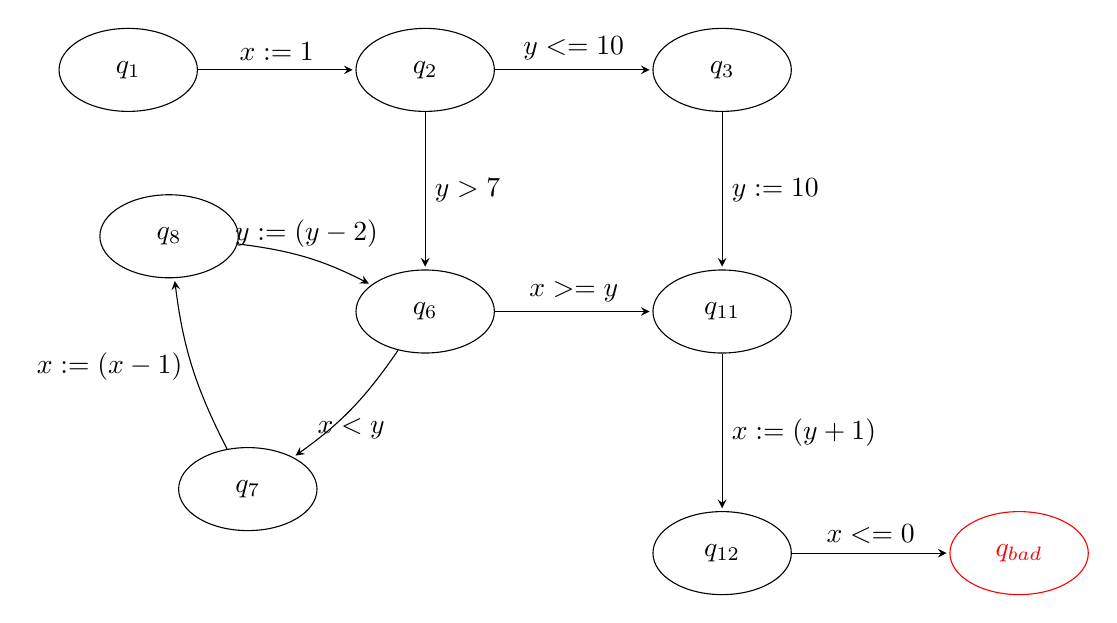
\begin{tikzpicture}[%
    ->,
    shorten >=1pt,
    >=stealth,
    node distance=7cm,
    noname/.style={%
      ellipse,
      minimum width=5em,
      minimum height=3em,
      draw
    }
  ]
    \node[noname] (1)                                   {$q_{1}$};
    \node[noname] (2) [node distance=2cm,right=of 1]    {$q_{2}$};
    \node[noname] (3) [node distance=2cm,right=of 2]    {$q_{3}$};
    \node[noname] (6) [node distance=2cm,below=of 2]    {$q_{6}$};
    \node[noname] (7) [node distance=1.5cm and 1cm,below left=of 6]    {$q_{7}$};
    \node[noname] (8) [node distance=0.2cm and 2,above left=of 6]    {$q_{8}$};
    \node[noname] (11) [node distance=2cm,below =of 3]   {$q_{11}$};
    \node[noname] (12) [node distance=2cm,below=of 11]   {$q_{12}$};
    \node[noname, red] (bad) [node distance=2cm,right=of 12]   {$q_{bad}$};

    \path (1) edge  [above]                  node {$x := 1$}   (2)
          (2) edge  [above]                  node {$y <= 10$}  (3)
          (2) edge  [right]                  node {$y >7$}    (6)
          (3) edge  [right]                  node {$y := 10$}  (11)
          (6) edge  [bend left=10pt, below]  node {$x < y$}    (7)
          (6) edge  [above]                  node {$x >= y$}   (11) 
          (7) edge  [bend left=10pt, left]   node {$x := (x-1)$} (8)
          (8) edge  [bend left=10pt, above]  node {$y := (y-2)$} (6)
          (11) edge [right]                  node {$x := (y+1)$} (12)
          (12) edge [above]                  node {$x <= 0$}     (bad)
          ;
  \end{tikzpicture}
\paragraph{Expected result}$\exists B_0$ such that:
\begin{itemize}
\item $\forall $ \texttt{bound} $< B_0 \rightarrow$ No feasible path of length $\leq 10$.
\item $\forall $ \texttt{bound} $\geq B_0 \rightarrow$: A path to the final state.
\end{itemize}

\paragraph{Obtained result}
For a bound of 26 a feasible path is found.\\
\textbf{\textcolor{teal}{PASS}}

\subsubsection{Recognising fixed points}
\paragraph{Test File:} \texttt{loop\_never\_sat.aut}

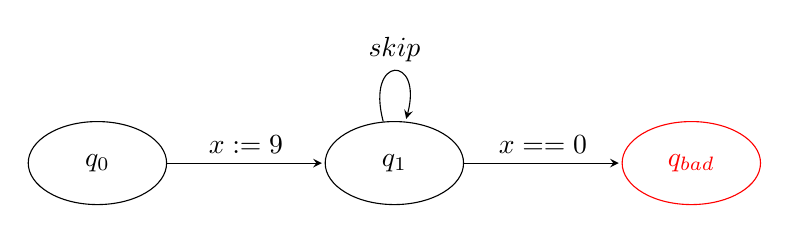
\begin{tikzpicture}[%
    ->,shorten >=1pt,>=stealth,node distance=7cm,noname/.style={%
      ellipse,minimum width=5em, minimum height=3em,draw}
  ]
    \node[noname] (ini)                                        {$q_{0}$};
    \node[noname] (1) [node distance=2cm, right=of ini]        {$q_{1}$};
    \node[noname, red] (bad) [node distance=2cm, right=of 1]   {$q_{bad}$};
    \path (ini) edge [above]                  node {$x:=9$}  (1)
    	  (1)   edge [loop above]             node {$skip$} (1)
          (1)   edge [above]                  node {$x==0$}   (bad)
          ;
  \end{tikzpicture}
\paragraph{Test}
If a program that is safe contains a loop, whatever the chosen bound, no feasible path of length $\leq $ \texttt{bound} is found.


\paragraph{Expected result}
$\forall $ \texttt{bound} $\rightarrow$ no feasible path of length $\leq $\texttt{bound}.
\paragraph{Obtained result}
No path of length $\leq 1000$ is found.
 
\textbf{\textcolor{teal}{PASS}}

\paragraph{Remark}
The bounded model checker will never prove that a program that contains loops is safe. It will only prove that there are are no paths of length $\leq$ \texttt{bound} to the final location. The objective of a bounded model checker is to find bugs, and not necessarily to prove that the system is safe, so we can consider this to be expected behaviour even though, to a human eye, it is evident that this program is safe, regardless of the bound.

This test demonstrates that the bounded model checker gets stuck in a loop\footnote{The model checker will only loop until the bound is reached.} if the state is the same as a previously encountered one. Therefore if a location has been visited and the solver obtained when reaching this location is equivalent to a solver previously obtained at this location, the depth first search still propagates.

Consequently, even though a program is safe, the bounded model checker will often only be able to guarantee that there is no path to the final location of length lower or equal to \texttt{bound}, for any positive bound.

\subsection{Existing Automaton examples}
\subsubsection{Division by zero}
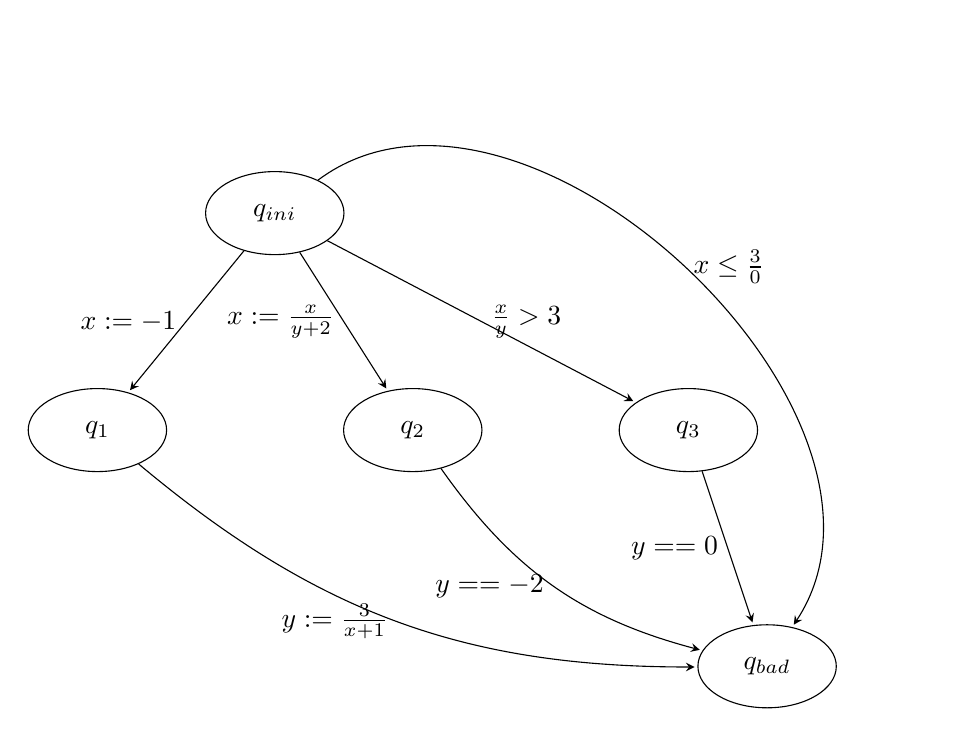
\begin{tikzpicture}[%
    ->,
    shorten >=1pt,
    >=stealth,
    node distance=7cm,
    noname/.style={%
      ellipse,
      minimum width=5em,
      minimum height=3em,
      draw
    }
  ]
    \node[noname] (ini)                                                {$q_{ini}$};
    \node[noname] (1) [node distance=2cm and 1cm,below left=of ini]    {$q_{1}$};
    \node[noname] (2) [node distance=2cm and 0.5cm,below right=of ini] {$q_{2}$};
    \node[noname] (3) [node distance=2cm and 4cm,below right=of ini]   {$q_{3}$};
    \node[noname] (bad) [node distance=5cm and 5cm,below right=of ini]   {$q_{bad}$};

    \path (ini) edge [left]                  node {$x:=-1$} (1)
          (ini) edge [left]                  node {$x:=\frac{x}{y+2}$} (2)
          (ini) edge [right]                  node {$\frac{x}{y} > 3$} (3)
          (ini) edge [bend left=80pt, right] node {$x \leq \frac{3}{0}$} (bad)
          (1)   edge [bend right=20pt, left] node {$y:=\frac{3}{x+1}$} (bad)
          (2)   edge [bend right=20pt, left] node {$y == -2$} (bad)
          (3)   edge [left] node {$y==0$} (bad)
          ;
  \end{tikzpicture}
  
The division by zero automaton should not lead to a bad state, indeed 
\begin{itemize}
\item $q_{ini} \rightarrow q_1 $: enforces $x:=-1$, so we cannot have $y:=\frac{3}{x+1}$ we would have a division by zero, this produces an {\sc{unsat}} formula.
\item $q_{ini} \rightarrow q_2 $: enforces $x:=\frac{x}{y+2}$, so we cannot have $y==-2$.
\item $q_{ini} \rightarrow q_3 $: enforces $\frac{x}{y} > 3$, so we must have $y\neq 0$.
\item $q_{ini} \rightarrow q_{bad} $: dividing by zero produces an {\sc{unsat}} formula.
\end{itemize}  


The bounded model checker finds that there is no feasible path.

\textbf{\textcolor{teal}{PASS}}


\subsubsection{Constant Propagation}

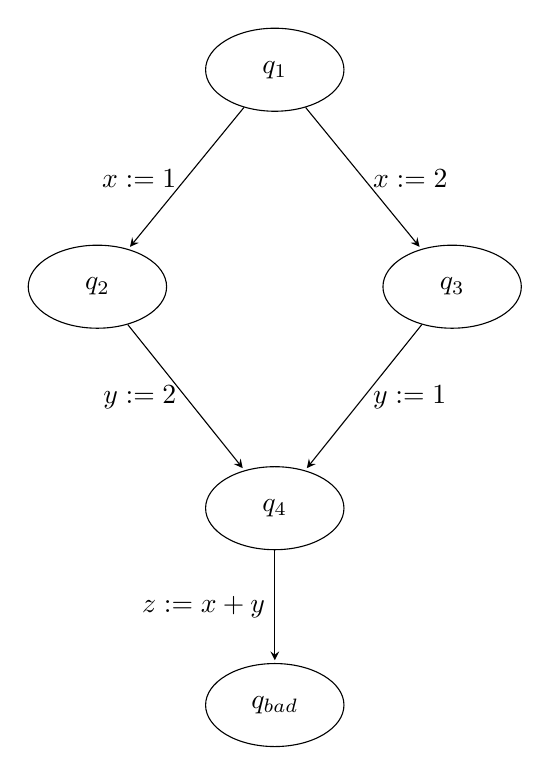
\begin{tikzpicture}[%
    ->,
    shorten >=1pt,
    >=stealth,
    node distance=7cm,
    noname/.style={%
      ellipse,
      minimum width=5em,
      minimum height=3em,
      draw
    }
  ]
    \node[noname] (1)                                                {$q_{1}$};
    \node[noname] (2) [node distance=2cm and 1cm,below left=of 1]    {$q_{2}$};
    \node[noname] (3) [node distance=2cm and 1cm,below right=of 1] {$q_{3}$};
    \node[noname] (4) [node distance=4.5cm,below =of 1]   {$q_{4}$};
    \node[noname] (bad) [node distance=7cm,below =of 1]   {$q_{bad}$};

    \path (1) edge [left]                   node {$x:=1$}   (2)
          (1) edge [right]                  node {$x:=2$}   (3)
          (2) edge [left]                   node {$y:=2$}   (4)
          (3) edge [right] 					node {$y:=1$}   (4)
          (4) edge [left]  					node {$z:=x+y$} (bad)
          ;
  \end{tikzpicture}

Clearly the constant propagation automaton is unsafe: for any initial value of x and y and for z=3, the final state $q_{bad}$ is reached. 

The bounded model checker finds the following feasible path to $q_{bad}$:

\begin{minted}{c}
Feasible path:
   q_1
     >> x := 1 >>
   q_2
      >> y := 2 >>
   q_4
      >> z := (x + y) >>
   q_5

\end{minted}

\textbf{\textcolor{teal}{PASS}}

\subsubsection{Inductive Invariants Exercise 1}
\begin{tikzpicture}[%
    ->,
    shorten >=1pt,
    >=stealth,
    node distance=7cm,
    noname/.style={%
      ellipse,
      minimum width=5em,
      minimum height=3em,
      draw
    }
  ]
    \node[noname] (0)                                      {$q_{0}$};
    \node[noname] (1)   [node distance=3cm, right=of 0]    {$q_{1}$};
    \node[noname] (bad) [node distance=8cm, right=of 0]    {$q_{bad}$};

    \path (0) edge [above]                    node {$x:=0$}       (1)
          (1) edge [loop above=80pt,above]    node {$x:=(x*y)$}   (1)
          (1) edge [loop below=100pt, below]  node {$x:=(x+3)$}   (1)
          (1) edge [above]  				  node {$x==10$}     (bad)
          ;
  \end{tikzpicture}
  
In this exercise we have a safe inductive invariant:
\begin{itemize}
\item $\varphi _{q_0}$ = true
\item $\varphi _{q_1}$ = $\exists k \in \mathbb{Z} : x = 3*k$
\item $\varphi _{q_{bad}}$ = false
\end{itemize}

The bounded model checker finds that there is no feasible path of length $\leq $ \texttt{bound}.

\textbf{\textcolor{teal}{PASS}}

\subsubsection{Inductive Invariants Exercise 2}

\begin{tikzpicture}[%
    ->,
    shorten >=1pt,
    >=stealth,
    node distance=7cm,
    noname/.style={%
      ellipse,
      minimum width=5em,
      minimum height=3em,
      draw
    }
  ]
    \node[noname] (0)                                                {$q_{0}$};
    \node[noname] (1) [node distance=2cm,right=of 0]    {$q_{1}$};
    \node[noname] (2) [node distance=2cm,right=of 1] {$q_{2}$};
    \node[noname] (3) [node distance=2cm,right=of 2]   {$q_{3}$};
    \node[noname] (4) [node distance=2cm,below=of 2]   {$q_{4}$};
    \node[noname, red] (bad) [node distance=2cm,left=of 4]   {$q_{bad}$};

    \path (ini) edge [above]                  node {$y > 0$} (1)
          (1) edge [above]                    node {$x:=0$} (2)
          (2) edge [bend right=20pt,below]     node {$x:= (x+y)$} (3)
          (2) edge [right]   node {$y==0$} (4)
          (3) edge [bend right=20pt, above]   node {$y:=(y-1)$} (2)
          (4) edge [above]   node {$x==0$} (bad)
          ;
  \end{tikzpicture}

In this exercise we have a safe inductive invariant:
\begin{itemize}
\item $\varphi _{q_0}$ = true
\item $\varphi _{q_1}$ = $y > 0$
\item $\varphi _{q_2}$ = $(y>0 \Rightarrow x \geq 0) \wedge (y=0 \Rightarrow x>0)$
\item $\varphi _{q_3}$ = $(y\geq 0 \Rightarrow x > 0)$
\item $\varphi _{q_4}$ = $(y=0 \wedge x > 0)$
\item $\varphi _{q_{bad}}$ = false
\end{itemize}

The bounded model checker finds that there is no feasible path of length $\leq $ \texttt{bound}.

\textbf{\textcolor{teal}{PASS}}

\subsubsection{Running Example}
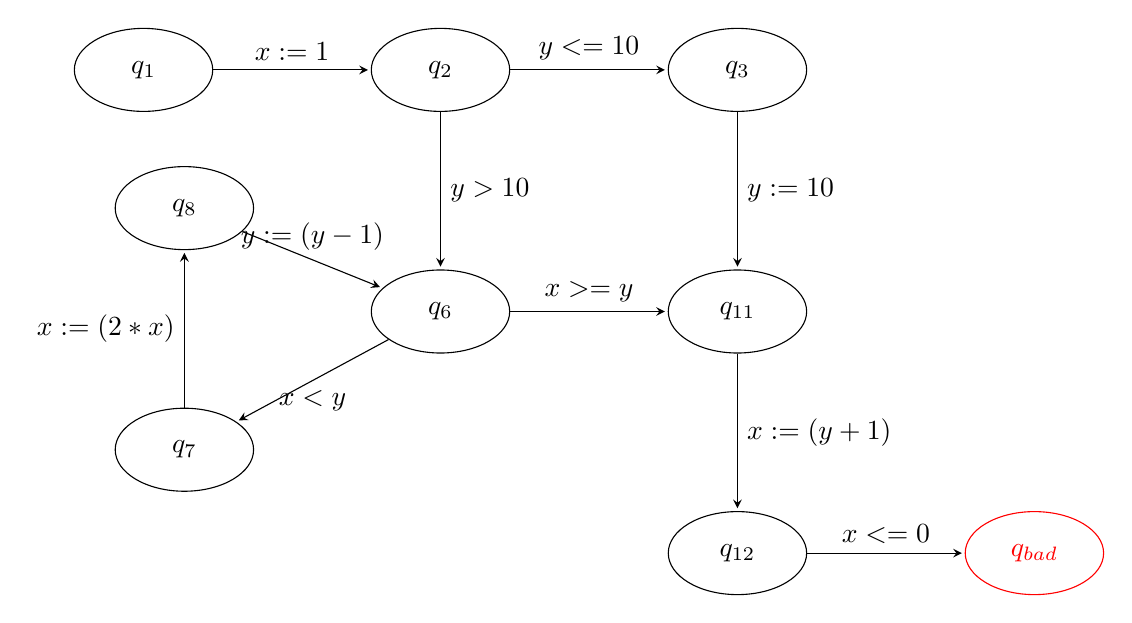
\begin{tikzpicture}[%
    ->,
    shorten >=1pt,
    >=stealth,
    node distance=7cm,
    noname/.style={%
      ellipse,
      minimum width=5em,
      minimum height=3em,
      draw
    }
  ]
    \node[noname] (1)                                   {$q_{1}$};
    \node[noname] (2) [node distance=2cm,right=of 1]    {$q_{2}$};
    \node[noname] (3) [node distance=2cm,right=of 2]    {$q_{3}$};
    \node[noname] (6) [node distance=2cm,below=of 2]    {$q_{6}$};
    \node[noname] (7) [node distance=1cm and 2cm,below left=of 6]    {$q_{7}$};
    \node[noname] (8) [node distance=2cm,above=of 7]    {$q_{8}$};
    \node[noname] (11) [node distance=2cm,below =of 3]   {$q_{11}$};
    \node[noname] (12) [node distance=2cm,below=of 11]   {$q_{12}$};
    \node[noname, red] (bad) [node distance=2cm,right=of 12]   {$q_{bad}$};

    \path (1) edge [above]                  node {$x:=1$} (2)
          (2) edge [above]                  node {$y<=10$} (3)
          (2) edge [right]                  node {$y>10$} (6)
          (3) edge [right]   node {$y:=10$} (11)
          (6) edge [below]   node {$x<y$} (7)
          (6) edge [above]   node {$x>=y$} (11) 
          (7) edge [left]   node {$x:=(2*x)$} (8)
          (8) edge [above]   node {$y:=(y-1)$} (6)
          (11) edge [right]   node {$x:= (y+1)$} (12)
          (12) edge [above]   node {$x<=0$} (bad)
          ;
  \end{tikzpicture}
  
With extended sign analysis it can be proved that this program is safe. The bounded model checker finds that there is no feasible path of length $\leq $ \texttt{bound}.

\textbf{\textcolor{teal}{PASS}}

\subsubsection{Infinite Descent}

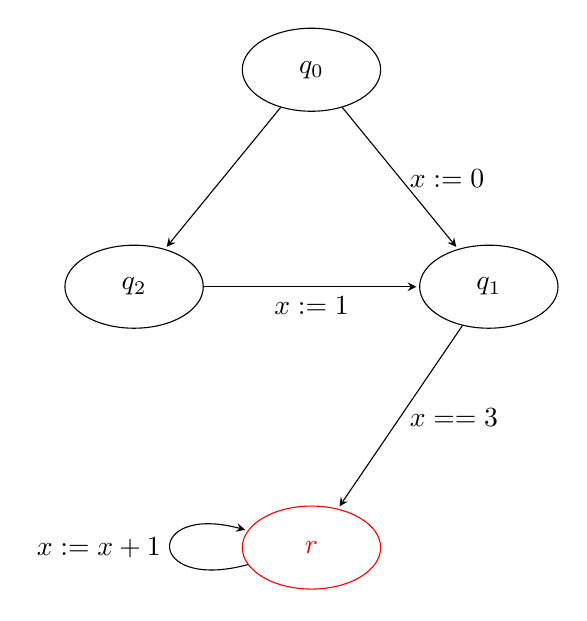
\begin{tikzpicture}[%
    ->,
    shorten >=1pt,
    >=stealth,
    node distance=7cm,
    noname/.style={%
      ellipse,
      minimum width=5em,
      minimum height=3em,
      draw
    }
  ]
    \node[noname] (0)                                                {$q_{0}$};
    \node[noname] (1) [node distance=2cm and 1cm,below right=of 0]   {$q_{1}$};
    \node[noname] (2) [node distance=2cm and 1cm,below left=of 0]    {$q_{2}$};
    \node[noname, red] (bad) [node distance=5cm,below=of 0]          {$r$};

    \path (0) edge []                    node {}       (2)
          (0) edge [right]                    node {$x:=0$} (1)
          (1) edge [right]    node {$x == 3$} (bad)
          (2) edge [below]                    node {$x:=1$} (1)
          (bad) edge [loop left]                    node {$x:=x+1$} (bad)
          ;
  \end{tikzpicture}
  
Clearly this automaton has no feasible path, we have a safe inductive invariant:
\begin{itemize}
\item $\varphi _{q_0}$ = true
\item $\varphi _{q_1}$ = $(x=0) \vee (x=3)$
\item $\varphi _{q_2}$ = true
\item $\varphi _{q_{bad}}$ = false
\end{itemize}   
The bounded model checker also finds that there is no feasible path.

\textbf{\textcolor{teal}{PASS}}
\paragraph{Remark}Since the loop in this example is on the final location, the bounded model checker does not get stuck in the loop. Indeed if it were to reach the loop it would have reached the final location, and found a path to the final location.

\subsubsection{Pre Only}

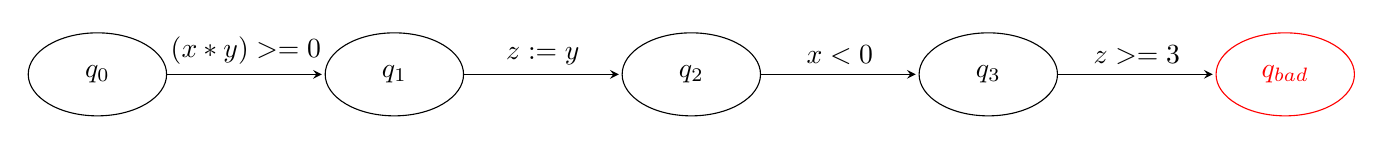
\begin{tikzpicture}[%
    ->,
    shorten >=1pt,
    >=stealth,
    node distance=7cm,
    noname/.style={%
      ellipse,
      minimum width=5em,
      minimum height=3em,
      draw
    }
  ]
    \node[noname] (0)                                                {$q_{0}$};
    \node[noname] (1) [node distance=2cm, right=of 0]   {$q_{1}$};
    \node[noname] (2) [node distance=2cm, right=of 1]    {$q_{2}$};
    \node[noname] (3) [node distance=2cm, right=of 2]    {$q_{3}$};
    \node[noname, red] (bad) [node distance=2cm,right=of 3]          {$q_{bad}$};

    \path (0) edge [above]                    node {$(x*y) >= 0$}       (1)
          (1) edge [above]                    node {$z:=y$} (2)
          (2) edge [above]                     node {$x<0$} (3)
          (3) edge [above]                    node {$z>=3$} (bad)
          ;
  \end{tikzpicture}

In this test we have a safe inductive invariant:
\begin{itemize}
\item $\varphi _{q_0}$ = true
\item $\varphi _{q_1}$ = $((x\geq 0) \wedge (y\geq 0)) \vee ((x\leq 0 )\wedge( y\leq 0))$
\item 
$\varphi _{q_2}$ = $((x\geq 0) \wedge (y\geq 0)) \vee ((x\leq 0 )\wedge( y\leq 0)) \bigwedge (z=y)$ \\
$\Leftrightarrow \varphi _{q_2}$ =$((x\geq 0) \wedge (z\geq 0)) \vee ((x\leq 0 )\wedge( z\leq 0)) \bigwedge (z=y)$
\item $\varphi _{q_3}$ = $((x < 0 )\wedge( z\leq 0)) \bigwedge (z=y)$
\item $\varphi _{q_{bad}}$ = false
\end{itemize}   

The bounded model checker also finds that there is no feasible path.

\textbf{\textcolor{teal}{PASS}}

\subsubsection{Sign Non Zero Crucial}
\begin{tikzpicture}[%
    ->,
    shorten >=1pt,
    >=stealth,
    node distance=7cm,
    noname/.style={%
      ellipse,
      minimum width=5em,
      minimum height=3em,
      draw
    }
  ]
    \node[noname] (0)                                                {$q_{0}$};
    \node[noname] (1) [node distance=2cm and 1cm,below right=of 0]    {$q_{1}$};
    \node[noname] (2) [node distance=2cm, right=of 1] {$q_{2}$};
    \node[noname] (3) [node distance=2cm and 1cm,below left=of 0]   {$q_{3}$};
    \node[noname] (4) [node distance=5cm,below=of 0]   {$q_{4}$};
    \node[noname, red] (bad) [node distance=2cm,right=of 4]   {$q_{bad}$};

    \path (0) edge [right]                    node {$x >= 0$} (1)
          (0) edge [left]                    node {$x < 0$} (3)
          (1) edge [bend right=20pt,below]     node {$x<10$} (2)
          (1) edge [right]                   node {$x >= 10$} (4)
          (2) edge [bend right=20pt, above]   node {$x:=(x+1)$} (1)
          (3) edge [loop left]   node {$x:=(x-1)$} (3)
          (3) edge [left]   node {$x<=10$} (4)
          (4) edge [above]   node {$x==0$} (bad)
          ;
  \end{tikzpicture}
  
  
In this test we have a safe inductive invariant:
\begin{itemize}
\item $\varphi _{q_0}$ = true
\item $\varphi _{q_1}$ = $(x\geq 0)$
\item $\varphi _{q_2}$ = $(x\geq 0) \wedge (x<10)$
\item $\varphi _{q_3}$ = $(x < 0)$
\item $\varphi _{q_4}$ = $(x < 0 )\vee( x\geq 10)$
\item $\varphi _{q_{bad}}$ = false
\end{itemize}   

The bounded model checker also finds that there is no feasible path of length $\leq$ \texttt{bound}.
 
\textbf{\textcolor{teal}{PASS}}
 
\subsubsection{Sign Non Zero Crucial Variant}
\begin{tikzpicture}[%
    ->,
    shorten >=1pt,
    >=stealth,
    node distance=7cm,
    noname/.style={%
      ellipse,
      minimum width=5em,
      minimum height=3em,
      draw
    }
  ]
    \node[noname] (0)                                                {$q_{0}$};
    \node[noname] (1) [node distance=2cm and 1cm,below right=of 0]    {$q_{1}$};
    \node[noname] (2) [node distance=2cm, right=of 1] {$q_{2}$};
    \node[noname] (3) [node distance=2cm and 1cm,below left=of 0]   {$q_{3}$};
    \node[noname] (4) [node distance=5cm,below=of 0]   {$q_{4}$};
    \node[noname, red] (bad) [node distance=2cm,right=of 4]   {$q_{bad}$};

    \path (0) edge [right]                    node {$x:=2$} (1)
          (0) edge [left]                    node {$x:=-3$} (3)
          (1) edge [bend right=20pt,below]     node {$x<10$} (2)
          (1) edge [right]                   node {$x >= 10$} (4)
          (2) edge [bend right=20pt, above]   node {$x:=(x+1)$} (1)
          (3) edge [loop left]   node {$x:=(x-1)$} (3)
          (3) edge [left]   node {$x<=10$} (4)
          (4) edge [above]   node {$x==0$} (bad)
          ;
  \end{tikzpicture}
  
In this test we have a safe inductive invariant:
\begin{itemize}
\item $\varphi _{q_0}$ = true
\item $\varphi _{q_1}$ = $(x > 0)$
\item $\varphi _{q_2}$ = $(x > 0)\wedge(x < 10)$
\item $\varphi _{q_3}$ = $(x < 0)$
\item $\varphi _{q_4}$ = $(x < 0)\vee(x \geq 10)$
\item $\varphi _{q_{bad}}$ = false
\end{itemize}   

The bounded model checker also finds that there is no feasible path of length $\leq$ \texttt{bound}.
 
\textbf{\textcolor{teal}{PASS}}
\end{document}
